\documentclass{article}
\usepackage[utf8]{inputenc}
\usepackage{setspace}
\usepackage{tikz}
\usetikzlibrary{positioning}
\usepackage{amsfonts}
\usepackage{amssymb}
\usepackage{amsmath}
\usepackage{amsthm}
\usepackage{systeme}
\usepackage{mathtools}
\usepackage{hyperref}
\usepackage{venndiagram}
\usepackage{pgfplots}
\usepgfplotslibrary{statistics}
\pgfplotsset{compat=1.18}
\usepackage{graphicx}
\usepackage{float}

\begin{document}

\section*{Question 1}

~

\subsection*{a}

~

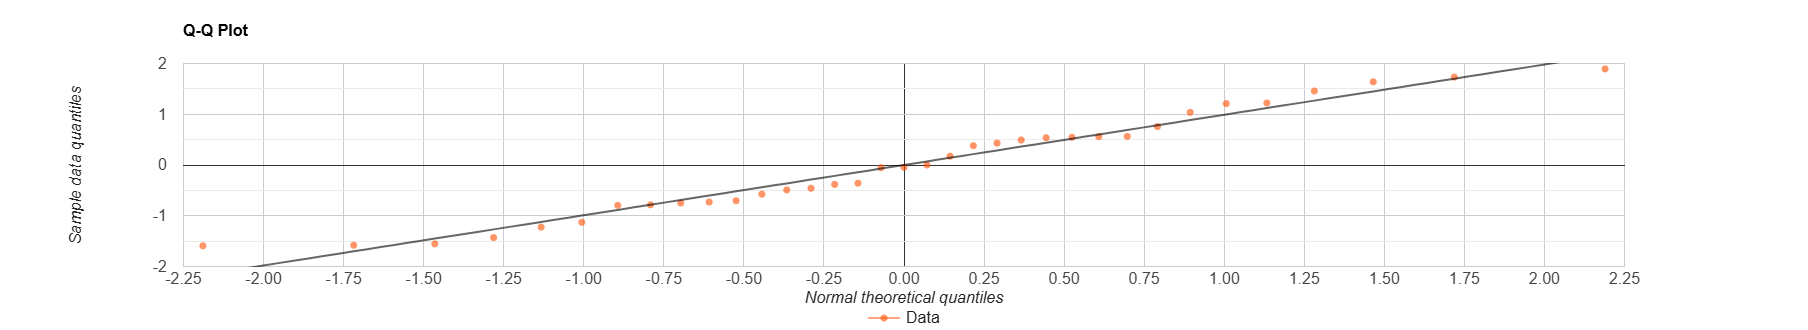
\includegraphics[scale=0.18]{1a.png}

The plot suggests that assumption of normal is acceptable.

\begin{align*}
    &H_0:{\sigma_1}^2={\sigma_2}^2={\sigma_3}^2={\sigma_4}^2={\sigma_5}^2\\
    &H_a:\exists i,j\in\{1,2,3,4,5\}:{\sigma_i}^2\ne{\sigma_j}^2\\
    &\text{Use Levene's test}:\\
    &f_{Levene}=\frac{\frac{\sum_{i=1}^{k}N_i(Z_{i\centerdot }-Z_{\centerdot \centerdot })^2}{k-1}}{\frac{\sum_{i=1}^{k}\sum_{j=1}^{N_1}(Z_{ij }-Z_{i \centerdot })^2}{N-k}}\\
    &f_{Levene}\geqslant F_{a,(k-1,N-k)}:H_0\text{ fails}\\
\end{align*}

~

\subsection*{b}

~

\begin{align*}
    &\alpha=0.01\\
    &Z_{ij}=|Y_{ij}-\overline{Y{i\centerdot}}|\\
    &\\
\end{align*}

\begin{table}[H]
    \begin{tabular}{|l|l|l|l|l|l|l|l|l|}
    \hline
            &       &       &       &       &       &       &       & $\overline{Y_{i\centerdot}}$ \\ \hline
    4 inch  & 309.2 & 409.5 & 311.0 & 326.5 & 316.8 & 349.8 & 309.7 & 333.21                     \\ \hline
    6 inch  & 402.1 & 347.2 & 361.0 & 404.5 & 331.0 & 348.9 & 381.7 & 368.06                     \\ \hline
    8 inch  & 392.4 & 366.2 & 351.0 & 357.1 & 409.9 & 367.3 & 382.0 & 375.13                     \\ \hline
    10 inch & 346.7 & 452.9 & 461.4 & 433.1 & 410.6 & 384.2 & 362.6 & 407.36                     \\ \hline
    12 inch & 407.4 & 441.8 & 419.9 & 410.7 & 473.4 & 441.2 & 465.8 & 437.17                     \\ \hline
    \end{tabular}
\end{table}

\begin{table}[H]
    \begin{tabular}{|l|l|l|l|l|l|l|l|l|}
    \hline
            &       &       &       &       &       &       &       & $Z_{i\centerdot}$ \\ \hline
    4 inch  & 24.01 & 76.29 & 22.21 & 6.71 & 16.41 & 16.59 & 23.51 & 26.53                     \\ \hline
    6 inch  & 34.04 & 20.86 & 7.06 & 36.44 & 37.06 & 19.16 & 13.64 & 24.04                     \\ \hline
    8 inch  & 17.27 & 8.93 & 24.13 & 18.03 & 34.77 & 7.83 & 6.87 & 16.83                    \\ \hline
    10 inch & 60.66 & 45.54 & 54.04 & 25.74 & 3.24 & 23.16 & 44.76 & 36.73                     \\ \hline
    12 inch & 29.77 & 4.63 & 17.27 & 26.47 & 36.23 & 4.03 & 28.63 & 21.00                     \\ \hline
    \end{tabular}
\end{table}

~

\begin{align*}
    &Z_{\centerdot\centerdot}=\frac{1}{N}\sum_{i=1}^{k}\sum_{j=1}^{N_i}Z_{ij}\\
    &=\frac{1}{35}\sum_{i=1}^{k}\sum_{j=1}^{N_i}Z_{ij}\\
    &=25.029\\
\end{align*}

\begin{table}[H]
    \begin{tabular}{|l|l|l|l|l|l|l|l|l|}
    \hline
            &       &       &       &       &       &       &       & $\sum_{j=1}^{N_i}(Z_{ij}-Z_{i\centerdot})^2$ \\ \hline
    4 inch  & 6.35 & 2475.16 & 18.67 & 392.85 & 102.42 & 98.98 & 9.12 & 3103.56                    \\ \hline
    6 inch  & 100.12& 10.11 & 288.31 & 153.91 & 169.53 & 23.81 & 108.03 & 853.82                    \\ \hline
    8 inch  & 0.19 & 62.47 & 53.23 & 1.43 & 321.80& 81.07 & 99.23 & 619.43                    \\ \hline
    10 inch & 572.28 & 77.58 & 299.57 & 120.82 & 1121.70 & 184.35 & 64.36 & 2440.67                     \\ \hline
    12 inch & 76.87 & 268.16 & 13.93 & 29.89 & 231.79 & 288.17 & 58.13 & 966.93                     \\ \hline
    \end{tabular}
\end{table}

~

\begin{align*}
    &f_{Levene}=\frac{\frac{\sum_{i=1}^{k}N_i(Z_{i\centerdot }-Z_{\centerdot \centerdot })^2}{k-1}}{\frac{\sum_{i=1}^{k}\sum_{j=1}^{N_1}(Z_{ij }-Z_{i \centerdot })^2}{N-k}}\\
    &=\frac{\frac{7((26.53-25.029)^2+...+(21-25.029)^2)}{5-1}}{\frac{3103.56+...+966.93}{35-5}}\\
    &=1.47\\
    &F_{0.01,(4,30)}=4.01\\
    &f_{Levene}<F_{0.01,(4,30)}\\
    \Rightarrow&H_0\text{ holds}\\
\end{align*}

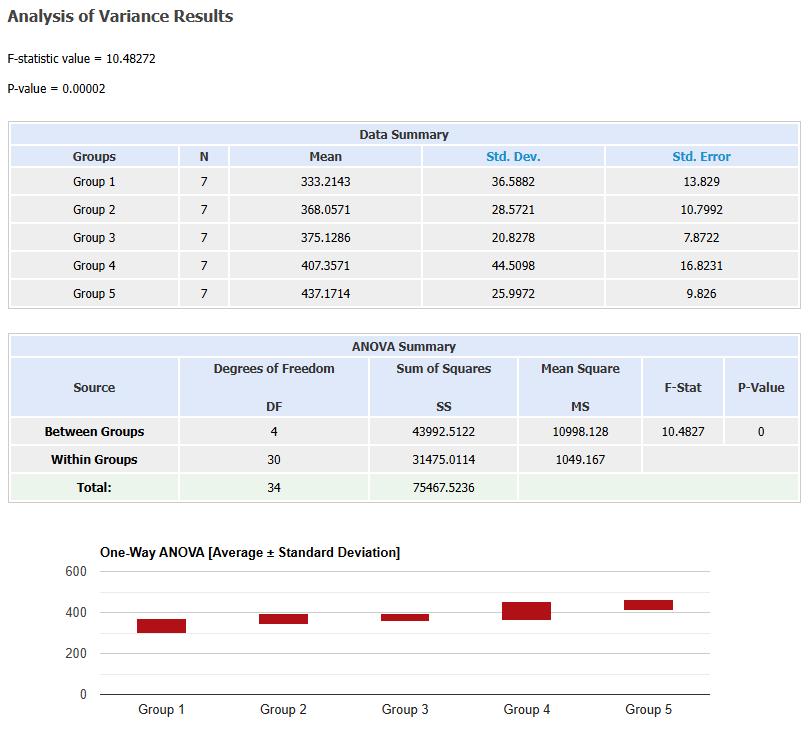
\includegraphics[scale=0.5]{1b.png}

\newpage

\section*{Question 2}

~

\subsection*{a}

~

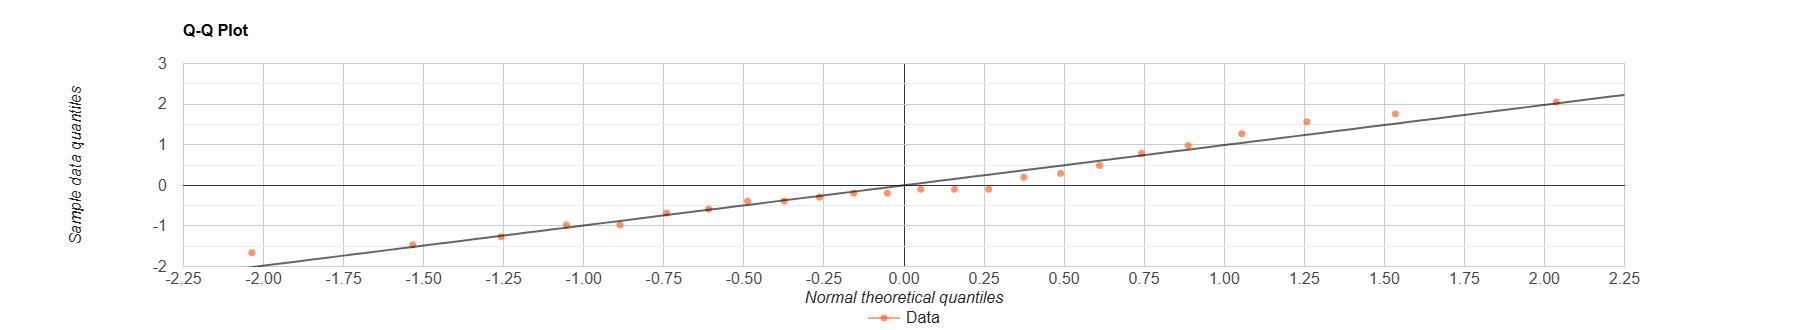
\includegraphics[scale=0.18]{2a.png}

The plot suggests that assumption of normal is acceptable.

\begin{align*}
    &H_0:{\sigma_1}^2={\sigma_2}^2={\sigma_3}^2={\sigma_4}^2\\
    &H_a:\exists i,j\in\{1,2,3,4\}:{\sigma_i}^2\ne{\sigma_j}^2\\
    &\text{Use P test}:\\
    &p\leqslant \alpha:\text{reject }H_0\\
\end{align*}

~

\subsection*{b}

~

\begin{align*}
    &T_1=34.3,T_2=39.6,T_3=33,T_4=41.9\\
    &G=T_1+T_2+T_3+T_4=148.8\\
    &N=24\\
    &\sum x^2=5.2^2+...+7.2^2=946.68\\
    &SS=\sum x^2-\frac{G^2}{N}=946.68-24\times148.8^2=24.12\\
    &SSB=\sum (\frac{T_1}{n}-\frac{G}{N})^2=8.98\\
    &SSW=SS-SSB=15.14\\
    &dfB=4-1=3\\
    &dfW=24-4=20\\
    &p=F_{0.05,(3,20)}=0.0229\\
    &0.0229<0.05\\
    \Rightarrow&\text{reject }H_0\\
    &\text{Thiamine content is not the same}\\
\end{align*}

\newpage

\section*{Question 3}

~

\subsection*{a}

~

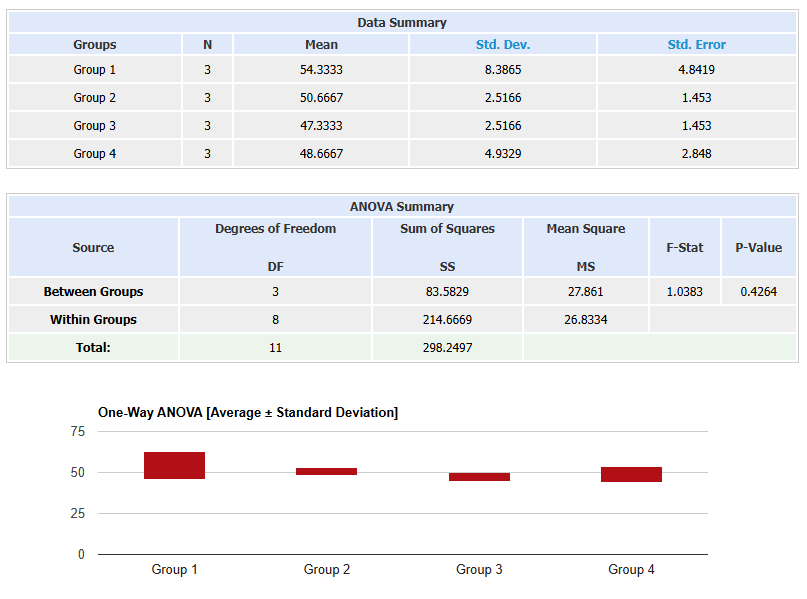
\includegraphics[scale=0.5]{3a.png}

\begin{align*}
    &H_0:{\sigma_1}^2={\sigma_2}^2={\sigma_3}^2={\sigma_4}^2\\
    &H_a:\exists i,j\in\{1,2,3,4\}:{\sigma_i}^2\ne{\sigma_j}^2\\
    &\overline{x_{1\centerdot}}=54.33,\overline{x_{2\centerdot}}=50.67,\overline{x_{3\centerdot}}=47.33,\overline{x_{4\centerdot}}=48.67,\overline{x_{\centerdot1}}=53.75,\overline{x_{\centerdot2}}=47,\overline{x_{\centerdot3}}=50\\
    &X_{\centerdot\centerdot}=603\\
    &\sum\sum{X_{ij}}^2=(64^2+...+52^2)=30599\\
    &CF=\frac{{X_{\centerdot\centerdot}}^2}{n}=\frac{603^2}{12}=30300.75\\
    &SS=\sum\sum{X_{ij}}^2=(64^2+...+52^2)-CF=30599-30300.75=298.25\\
    &SSB=\frac{1}{3}\sum{X_{i\centerdot}}^2-CF\\
    &=\frac{1}{3}(163^2+...+146^2)-30300.75\\
    &=83.58\\
    &SSW=\frac{1}{4}\sum{X_{\centerdot j}}^2-CF\\
    &=\frac{1}{4}(215^2+188^2+200^2)-30300.75\\
    &=91.5\\
    &SSE=SS-(SSB+SSW)=298.25-(83.58+91.5)=123.17\\
    &dfB=4-1=3\\
    &dfW=11-3=8\\
    &dfE=12-(3+2)=6\\
    &df=11\\
    &MSB=\frac{SSB}{dfB}=27.86\\
    &MSW=\frac{SSW}{dfW}=45.75\\
    &MSE=\frac{SSE}{dfE}=20.53\\
    &F_B=\frac{MSB}{MSE}=1.36\\
    &F_W=\frac{MSW}{MSE}=2.23\\
    &F_{0.05,(3,6)}=4.757\\
    \Rightarrow&F_B<F_{0.05,(3,6)}\\
    \Rightarrow&H_0\text{ holds}\\
\end{align*}

~

\subsection*{b}

~

\begin{align*}
    &\hat{\mu}=\overline{x_{\centerdot\centerdot}}=\frac{64+...+52}{12}=50.25\\
    &\hat{\alpha_1}=\overline{x_{1\centerdot}}-\overline{x_{\centerdot\centerdot}}=54.33-50.25=4.08\\
    &\hat{\alpha_2}=\overline{x_{2\centerdot}}-\overline{x_{\centerdot\centerdot}}=50.67-50.25=0.42\\
    &\hat{\alpha_3}=\overline{x_{3\centerdot}}-\overline{x_{\centerdot\centerdot}}=47.33-50.25=-2.92\\
    &\hat{\alpha_4}=\overline{x_{4\centerdot}}-\overline{x_{\centerdot\centerdot}}=48.67-50.25=-1.58\\
    &\hat{\beta_1}=\overline{x_{\centerdot1}}-\overline{x_{\centerdot\centerdot}}=53.75-50.25=3.5\\
    &\hat{\beta_2}=\overline{x_{\centerdot2}}-\overline{x_{\centerdot\centerdot}}=47-50.25=-3.25\\
    &\hat{\beta_3}=\overline{x_{\centerdot3}}-\overline{x_{\centerdot\centerdot}}=50-50.25=-0.25\\
\end{align*}

\newpage

\section*{Collaborators}

~

Frank Zhu

~

Jeffery Shu

~

Sam Sun

\end{document}